\chapter{Introduction of the ASE Template}
\label{chap:f}
\lipsum[1]

\begin{figure}[htp]
  \centering
  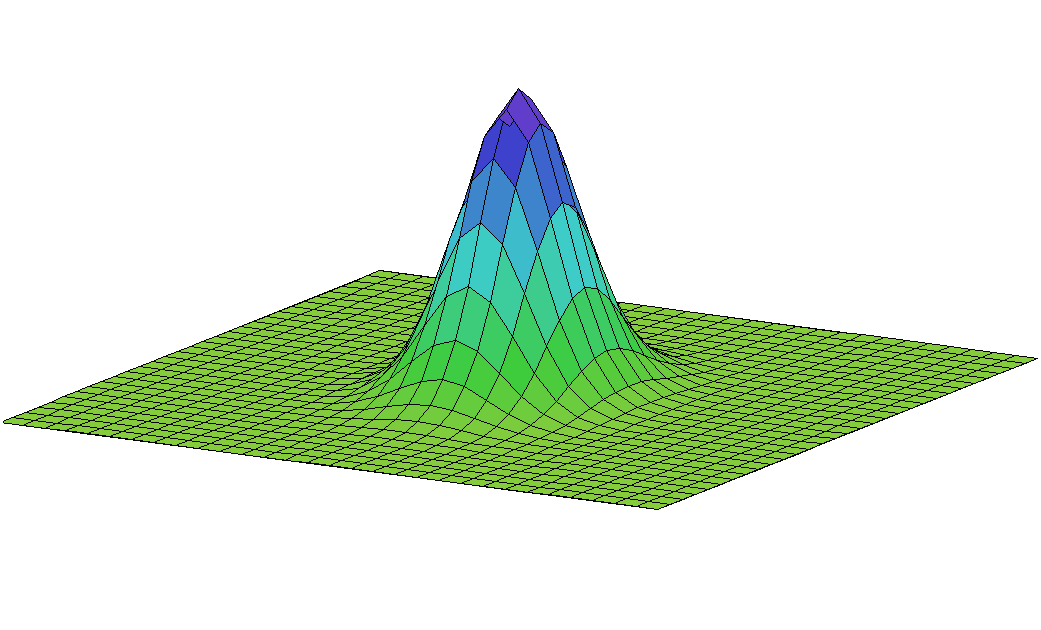
\includegraphics[width=6cm]{frontpage.png}
  \caption{Test of a picture}
  \label{fig:test}
\end{figure}

\lipsum[1]
\begin{figure}[ht]
  \begin{minipage}[htp]{0.48\linewidth}
    \centering
    \includegraphics[width=\linewidth]{ase_logo.png}
  \end{minipage}
  \hfill
  \begin{minipage}[htp]{0.48\linewidth}
    \centering
      \includegraphics[width=\linewidth]{ase_logo.png}
  \end{minipage}
    \caption{Pictures side by side}
  \label{fig:test1}
\end{figure}

\lipsum[1]

\section{Section dummy text}

\lipsum[1]

\[
 \frac{n!}{k!(n-k)!} = \binom{n}{k}
\]
\begin{equation}
  \frac{n!}{k!(n-k)!} = \binom{n}{k}
\end{equation}
\lipsum[1]

\subsection{Subsection dummy text}

\lipsum[1]

\begin{figure}
    \subfloat[Subcaption $1+a$]{\framebox[7cm]{First}} \hfill
    \subfloat[Subcaption $1+b$]{\framebox[7cm]{Second}}
    \caption{Main caption $1+x$} 
\end{figure}

\lipsum[1]
\section{Another dummy section}

\lipsum

Test of the reference system \cite{Rabiner89}.